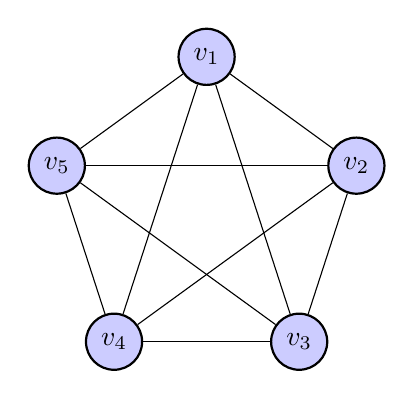
\begin{tikzpicture}
  [scale=1,auto=left,every node/.style={circle,fill=blue!20,draw=black,thick}]
  \node (n1) at (90:2) {$v_1$};
  \node (n2) at (18:2) {$v_2$};
  \node (n3) at (-54:2) {$v_3$};
  \node (n4) at (-126:2) {$v_4$};
  \node (n5) at (-198:2) {$v_5$};

  \foreach \from/\to in {n1/n2, n1/n3, n1/n4, n1/n5, n2/n3, n2/n4, n2/n5, n3/n4, n3/n5, n4/n5}
    \draw (\from) -- (\to);

 \end{tikzpicture}
